\chapter{绪论}

\section{研究背景和意义}

进入二十一世纪以来,人们表示和传递信息的媒介从文本、声音扩展到了图像、视频。如今视频已经成为人们生产和生活中不可缺少的部分。另一方面,在计算机技术和通信技术的推动下,人们对网络的依赖和要求也越来越高。
智能手机、平板电脑等移动设备的普及,Wi-Fi、4G等无线网络的覆盖,让人们能够随时随地访问互联网。这样的环境催生并促进了一项技术的蓬勃发展,这就是视频流媒体。

视频流媒体简单来说就是通过网络在线播放视频。所谓流媒体,是指音视频等多媒体数据通过网络以连续稳定的流的形式传输到客户端的一系列技术、协议和方法的总称。在视频流媒体中,视频数据从服务器连续不断地传输到客户端,客户端可以一边接收一边播放,无需等待整个文件发送完毕。与下载方式相比,这种采用流式传输的视频播放具有显著的优点\supercite{Li2002},包括:1)启动延迟大大缩短,用户可以在等待几秒或十几秒的缓冲后就立即开始观看;2)视频数据不在客户端长时间驻留,不仅节省了用户存储空间,也一定程度上避免了内容版权保护问题;3)支持数据的实时生成和获取,大大扩展了视频应用场景的范围。正是由于其优秀的特性,视频流媒体得到了广泛的应用,逐渐成为人们消费视频内容的主要形式\supercite{Chen2013}。

视频流媒体应用按照其对实时性要求的不同可以分为点播和直播两大类。在点播应用中,内容提供商将预先制作好的视频放在服务器上,并发布内容的描述信息和链接,用户选择自己感兴趣的内容请求播放相应的视频。典型的例子是在线视频网站,如国外的YouTube\footnote{https://www.youtube.com/}、Netflix\footnote{https://www.netflix.com/},国内的优酷\footnote{http://www.youku.com/}、乐视\footnote{http://www.le.com/}等。大多在线教育网站如Coursera\footnote{https://www.coursera.org/}、网易公开课\footnote{http://open.163.com/}等也属于视频点播类应用。在直播应用中,视频数据则是通过现场录制实时生成的,上传到流媒体服务器之后再即时分发给观看者,具有很强的时效性。这类应用包括现在互联网上正兴起的秀场、游戏、生活类直播软件,以及已经很成熟的远程监控、视频会议等等。直播应用往往也会把实时事件的内容存储起来,后续以点播的形式继续提供。

网络条件的改善,采集与播放设备的普及,使得视频流媒体应用进入了一个高速增长的时期。根据Cisco的一项预测\footnote{http://www.cisco.com/c/en/us/solutions/collateral/service-provider/ip-ngn-ip-next-generation-network/white\_paper\_c11-481360.html},从2014年到2019年,视频流量在所有互联网流量中的占比将从64\%上升至80\%。路透社的一篇报道\footnote{http://www.reuters.com/article/us-internet-consumers-cisco-systems-idUSKBN0EL15E20140610}指出,在美国这一比例在2018年即将达到83\%。可见,视频流媒体正迎来一个高峰期。

在前所未有的机遇同时,视频流媒体也面临着诸多挑战。一方面,网络状况变得越来越复杂,传输可用带宽不可预知,如何保证视频数据及时高效地发送给每个用户成为了一个需要考虑的问题。另一方面,大部分用户终端设备的计算能力还很低,而视频分辨率在不断增大,且编解码的复杂度也越来越高,用户收到视频数据后的解码和显示所需计算量越来越大,快速实时解码变得越来越困难。下面对这两大挑战进行具体说明。

首先,从网络状况来看,目前既有几百kb/s速度的拨号或3G上网,又有几十Mb/s速度的局域网或光纤接入,而且随着移动通信网与Internet的融合,无线与有线网络混联,使得带宽和信道质量更加不确定。在这样异构且波动的网络环境下,确定的视频流很难高效传输,也很难满足不同接入用户的需求。举例来说,如果设置一个较低的码率,则对应的视频质量不高,达不到带宽充足用户的满意度;而如果设置较高的码率,则对低带宽的用户或者在带宽波动较大的情况下,会导致视频无法流畅播放,带来不好的用户体验。即使是同一个用户,由于其所在网络环境会不时变化,如果视频数据以恒定的速率传输,观看体验几乎不可能达到最优。

其次,从用户终端来看,虽然前沿处理器计算能力不断在增强,但大部分用户的设备用的还是几年前的处理器,运算能力相当有限。尤其是对于智能手机和平板电脑而言,由于电池的制约,只能采用ARM架构的低功耗处理器。与此截然相反的是,现在的采集和显示设备像素成倍增加,视频分辨率早已突破了720p(1280x720)乃至1080p(1920x1080)的限制,向4K(3840x2160)发展。为了压缩这些高清和超高清的视频,视频编码的技术复杂度也越来越高。高分辨率的视频和高复杂度的编码技术,使得解码计算量大大增加。在通用处理器上的实时解码,成为了限制视频流媒体服务进一步改善的瓶颈。

考虑到视频流媒体的广泛应用,如何解决这些问题从而进一步改善流媒体服务质量,具有重要的现实意义。视频流媒体的研究既受到了工业界的关注,也成为了学术界的一大热点。

\section{研究框架和问题}

视频流媒体是视频与流媒体的结合,这个领域的研究也涉及包括编码和传输在内的多个子领域。视频流媒体的研究可以从系统模块的角度分为以下几个部分(参见图\ref{fig:research-framework}):

\begin{itemize}
	\item 数据源端的研究,一方面是进行高效的压缩编码,以尽可能少的数据表示尽可能高的视频质量;另一方面是提供具备灵活性的码流,支持码率的变化甚至考虑容错,等等。
	\item 传输过程的研究,即如何又快又好地将视频数据送给用户,包括改善网络状况以提高传输的吞吐量和可靠性,合理公平地利用带宽资源,根据带宽情况自适应地调整传输速率等。
	\item 客户终端的研究,即优化用户设备收到视频码流之后的播放阶段,包括如何快速解码,进行一些画质增强等后处理过程从而更好地显示,等等。
\end{itemize}

\begin{figure}[h]
	\centering
	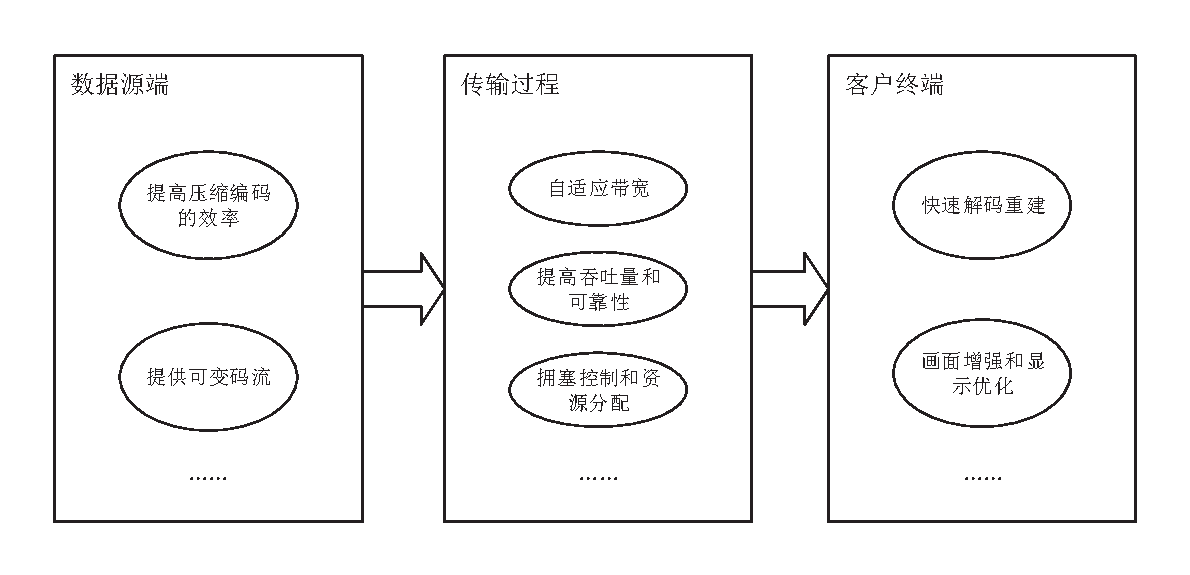
\includegraphics[width = 1.0\linewidth]{eps/research-framework}
	\caption{视频流媒体研究框架 \label{fig:research-framework}}
\end{figure}

数据源端对视频码流可变性的支持,再加上传输中自动调整码率以适应带宽的变化,结果就是所谓的自适应视频流媒体。在自适应视频流媒体中,服务器发送给客户端的视频流的码率能自动根据带宽的变化情况进行调整。这一特性能够很好地应对上一节中提到的网络异构和带宽波动带来的挑战。虽然其他方面的研究,例如对编码效率的提升、对网络架构和协议的改进,也非常重要,但本文主要关注的是自适应视频流媒体相关技术的研究。

通常有两种选择可以用来实现自适应视频流媒体。第一种选择是采取多码流的方法。多码流方法的原理很简单,就是预先编好不同码率的多个码流存放在服务器上,根据网络情况选取其中合适的一个进行传送。近年来兴起的HTTP动态自适应流媒体(Dynamic Adaptive Streaming over HTTP,  DASH)\supercite{Sodagar2011}就属于这类方法。如图\ref{fig:DASH}所示,DASH系统在服务器端提供不同码率的多个码流切片,客户端通过HTTP协议拉取数据,在某个时间段内可以选择性地接收这几个码流中任何一个的切片,通过在多码流之间切换来动态适应带宽波动。第二种选择是采用可伸缩视频编码\supercite{SVC-Overview}技术。作为国际视频编码H.264/AVC\supercite{H.264}的扩展之一,可伸缩视频编码目的就是在单个码流中加入伸缩性的支持,使其码率能够根据需要改变。因此,用它来实现自适应视频流媒体系统正符合其设计初衷。

\begin{figure}[t]
	\centering
	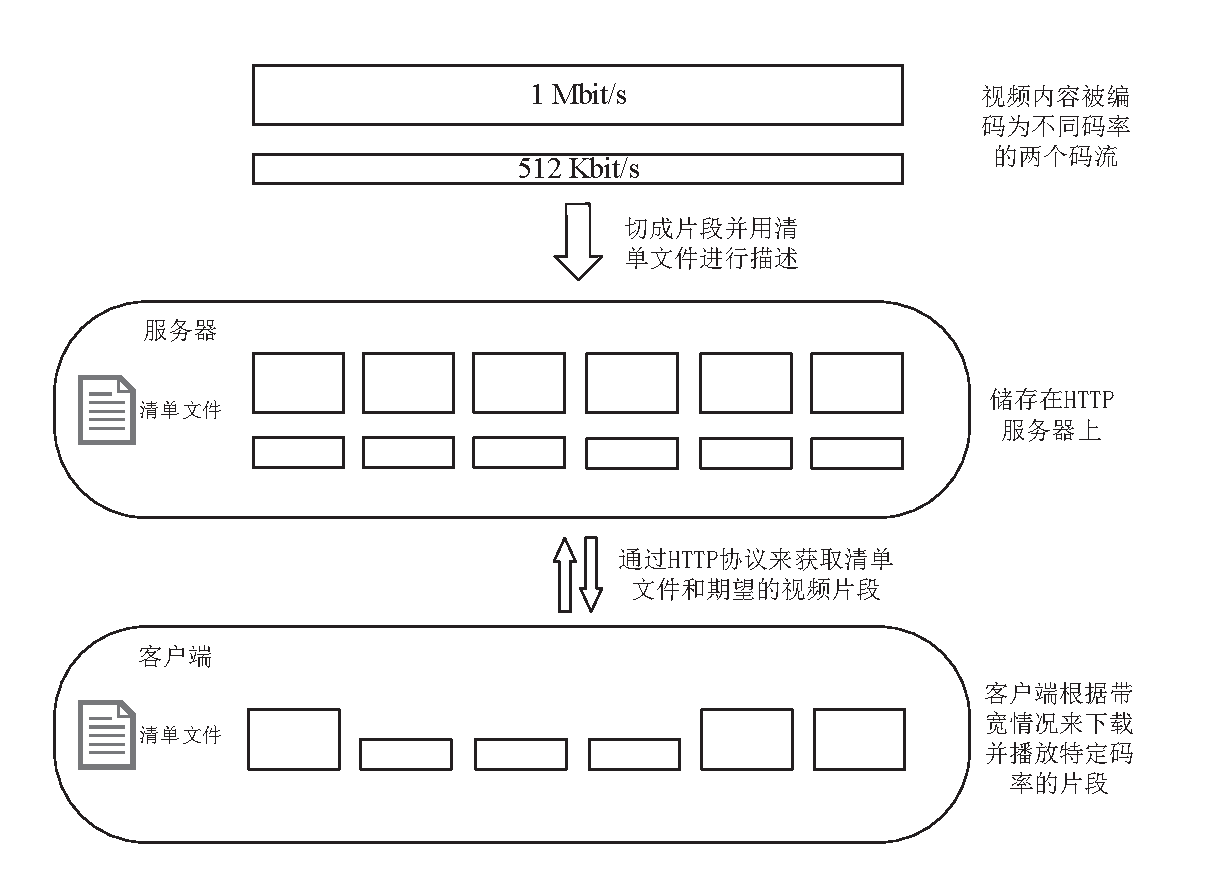
\includegraphics[width = 1.0\linewidth]{eps/DASH}
	\caption{DASH系统的工作原理示意图\label{fig:DASH}}
\end{figure}

多码流联播方案的优点是无需对已有的程序和系统做较大的改动,因此比较易于部署\supercite{Bouten2014}。很多商业视频网站(如YouTube、优酷等)已经用它实现了自适应功能。但是,多码流方案能提供的适应范围和粒度非常有限。例如,YouTube最多只提供240p、360p、480p、720p和1080p这五个等级,而优酷只提供标清、高清、超清这三个画质(参见图\ref{fig:13})。此外,多个码流的编码和存储需要大量的计算资源和磁盘空间,使得时间和空间开销成倍增加。要想以合理的代价提供精细无缝的自适应性,就需要采用可伸缩视频编码的方案。可伸缩视频码流能够以非常小的数据粒度进行码率调整,而且性能分析表明可伸缩视频编码的压缩效率远高于同一内容多次编码的多码流方法\supercite{SVC-Performance}。正是因为这些优势,采用可伸缩视频编码来实现自适应视频流媒体从技术上来说是一个更好的方案,也吸引了学术界很多研究者的关注\supercite{Chuah2012, Zhu2013, Dan2013, Yang2014, Cicalo2014}。

\begin{figure}[t]
	\centering
	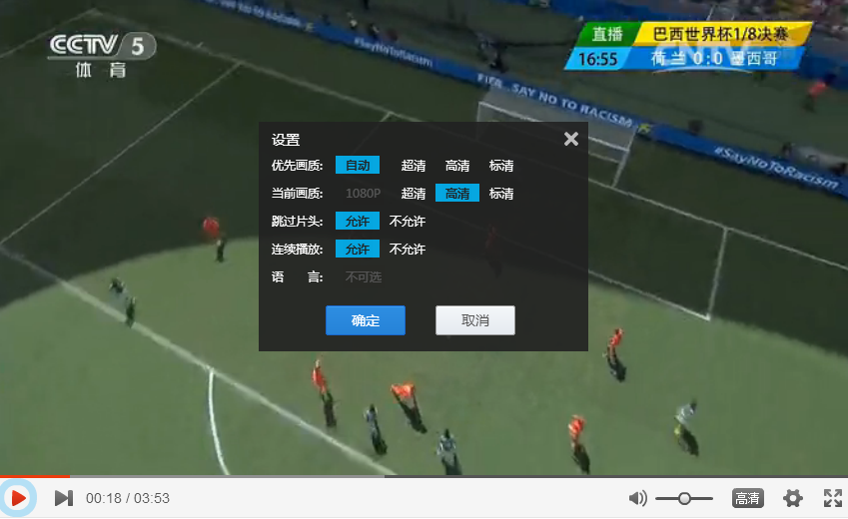
\includegraphics[width = 1.0\linewidth]{clip/13.png}
	\caption{优酷网视频码率自适应功能图示\label{fig:13}}
\end{figure}

从图\ref{fig:research-framework}所示的研究框架中可以看出,采用可伸缩视频编码或是采用DASH之类的多码流方案,其区别只在于数据源端提供灵活码流的方式不同。可伸缩视频作为数据源时,在给定码率下如何最优地从整个码流中截取出一个子流用于发送是需要研究的问题之一,DASH系统则不存在这个问题。而对于在传输中如何自动调整码率以适应带宽的变化,却是二者共有的问题。此外,无论是何种视频流媒体系统,当用户设备收到视频流后都需要进行解码和播放。为了在计算资源有限的设备上满足实时播放的要求,通用处理器上的解码优化也是值得重视的问题之一。这些问题的解决,是提高视频流媒体服务质量和用户体验的关键。

\section{本文研究内容和主要贡献}

本文结合视频流媒体所面临的挑战,对上面提到的关键问题进行研究。首先,本文针对可伸缩视频数据源提出了新的失真模型和码流截取方案,在支持可变码率的同时提供尽可能高的视频质量;其次,本文为视频数据的传输过程设计了新的码率自动调整策略,用控制论的方法来解决适应带宽变化的问题;最后,为了保证用户终端收到码流后能够快速实时的解码并播放,本文研究了新一代国际视频编码标准HEVC(High Efficiency Video Coding)\supercite{HEVC-Overview}的解码过程,提出了新的优化算法来对其进行加速。本文主要的创新性贡献可以归纳为如下三个部分:
\begin{enumerate}
\item {采用线性误差模型的码流截取方案}\\
作为码率适应带宽波动的前提条件,视频流媒体中的数据源需要能够灵活调整。可伸缩视频编码将数据划分为基本层和增强层,通过丢弃增强层的数据包来实现即时码率变化。从完整的可伸缩码流中丢弃部分数据得到一个子流的过程称为码流截取。本文以最小化特定截取码率限制下的视频失真为目标,首先提出了一个线性误差模型来估计丢弃任意数据包组合带来的失真变化,然后利用它设计了一个贪心型算法来根据每个数据包的码率和失真影响对其赋优先级,作为截取过程中丢包的顺序。相比于参考软件,这一码流截取方案能够以更低的复杂度取得更高的视频质量。
\item {基于PID控制思想的码率自适应算法}\\
自适应流媒体的另一个关键问题是传输过程中的码率调整策略,即在可用带宽不断变化的情况下,决定何时调整码率并确定调整到多少。本文基于经典的比例-积分-微分(Proportional-Integral-Derivative,PID)控制思想,提出了一个综合考虑带宽的历史状况、当前状态和未来趋势的码率自适应算法,既能充分利用带宽,传输较高的视频质量,又能减小带宽波动的影响,保证视频质量的平滑性。该算法在点播和直播的实际测试中都表现出了很好的性能,而且很容易扩展到各种自适应流媒体系统。
\item {高度优化的HEVC解码器设计与实现}\\
视频流媒体的最后一个阶段是码流在用户终端设备上的解码播放。为此,本文设计并实现了一个高度优化的HEVC软件解码器,将数据级和任务级并行方法相结合,显著提高了各个解码模块的计算效率以及整体解码速度。该解码器分别在主流的桌面和移动处理器上达到了4K ($3840 \times 2160$) 和720p ($1280 \times 720$) 视频的实时解码要求,并已成功应用于业界知名的视频流媒体平台迅雷看看,为进一步改善用户在线观看视频的体验提供了技术支撑。
\end{enumerate}

\section{本文的结构安排}

本文共分为六章,后续章节具体内容安排如下。

第二章概述视频流媒体领域的研究基础和相关工作。首先对视频编码和流式传输的基础知识进行简要介绍,为后文内容做准备;然后结合本文的研究内容对码流截取、码率自适应、解码器优化这几个问题和已有工作进行分析。

第三章讨论采用线性误差模型的码流截取方案。首先针对可伸缩视频推导并验证线性误差模型,然后介绍采用该模型的失真估计方法和以码率失真影响为度量标准的优先级赋值算法。最后展现并分析所提出的码流截取方案的实验结果。

第四章讨论基于PID控制思想的码率自适应算法。首先对PID控制器做简单的介绍,然后将PID模型运用到视频传输中的码率自适应问题,提出了一个新颖的码率自适应算法。该算法被集成在了实际点播和直播流媒体系统中,其有效性通过对比实验得到了验证。

第五章讨论针对新一代视频编码标准HEVC的解码优化工作。以重新设计的解码器原型为基础,首先采用单指令多数据技术对特定解码模块进行加速,然后引入帧级并行解码框架提高了在多核处理器上进行多线程解码的速度,最后对上述方法所取得的优化效果进行了评测。

第六章总结全文内容并对未来工作和应用前景进行展望。